\begin{center}
\textit{by Jonathan Kozaczuk, Andrew J. Long, Jose Miguel No, and Michael J. Ramsey-Musolf}
\end{center}

\noindent{\it Introduction.} Explaining the origin of the cosmic matter-antimatter asymmetry is a key open problem at the interface of high energy physics and cosmology. A number of scenarios have been proposed, ranging in energy scales from $\sim 10^{12}$ and above to below the electroweak scale and corresponding to different eras in cosmic history. One of the most compelling -- electroweak baryogenesis --  ties the generation of the asymmetry to electroweak symmetry breaking (for a review, see Ref.~\cite{Morrissey:2012db}). In this scenario, the universe must have undergone a first order phase from the electroweak symmetric to broken phase at a temperature $T_\mathrm{EW} \sim 100$ GeV. If such a transition occurred, then there must have also existed sufficiently active CP-violating interactions to produce the observed asymmetry. Neither requirement is satisfied by the Standard Model. The symmetry-breaking transition for a 125 GeV Higgs boson is known to be of a crossover type, and the CP-violating interactions encoded in the Cabibbo-Kobayashi-Maskawa matrix are too feeble to have produced the observed asymmetry. Thus, viable electroweak baryogenesis (EWBG) requires physics beyond the standard model that couples to the Higgs boson.

The HE LHC would provide new opportunities to search for this BSM physics. Studies of di-Higgs production, measurements of the Higgs triple self-coupling, and precision tests of other Higgs couplings are particularly interesting as probes of the new interactions needed for a first order electroweak phase transition (EWPT). For the first order phase transition to be sufficiently strong, so as to provide the needed conditions for EWBG, the new interactions must be mediated by particles with masses below roughly one TeV, making them accessible to $pp$ collisions at $\sqrt{s} = 27$ TeV. While a definitive program of searching for these interactions would likely require higher center of mass energy, the HE LHC would significantly extend the discovery reach over what is accessible at the HL LHC. Below, we provide a few key examples that illustrate this possibility.

\noindent{\it Higgs Potential at Finite Temperature.} The nature of the EWSB transition is governed by the temperature-dependent Higgs potential, $V_\mathrm{EFF}(\varphi, T)$. In the regime where $T\gg M_W$, this potential takes the 
simple form
\begin{equation}
V_\mathrm{EFF}(\varphi,T) = D(T^2-T_0^2)\varphi^2 -(ET+e)\varphi^3 + {\bar\lambda}\varphi^4+\cdots ~~.
\label{eq:HiggspotT}
\end{equation}
In the SM one has $e=0$, while $D$, $T_0$, $E$ and ${\bar\lambda}$ are all non-vanishing functions of the zero temperature parameters of the theory (e.g., gauge, Yukawa, and Higgs self-couplings). At any temperature, the minimum of energy is obtained when $\varphi$ equals its vacuum expectation value $v(T)$, with $v(0) = 246$ GeV. The Higgs boson field is just the difference $h=\varphi-v(0)$. 

At sufficiently high temperatures, the minimum of the potential resides at the origin, {\it i.e.}, $v(T) = 0$. As the universe cools, however, the minimum eventually moves away from the origin, corresponding to the onset of EWSB. The details of this evolution, and the nature of the transition (first order, second order, or crossover) depends on the values of the couplings in Eq.~(\ref{eq:HiggspotT}). Since the latter are determined by the $T=0$ interactions, measurements of Higgs boson properties allow one to infer the thermal history of electroweak symmetry breaking. 

Assuming the SM form of the $T=0$ Higgs potential and Higgs couplings to other SM particles, lattice studies imply that for a 125 GeV Higgs boson, the symmetry-breaking transition is of a cross over type\cite{Rummukainen:1998as,Csikor:1998eu,Laine:1998jb,Gurtler:1997hr}. Thus, one of the three \lq\lq Sakharov conditions" for successful baryogenesis\cite{Sakharov:1967dj} -- out of equilibrium dynamics -- would not have been satisfied, thereby precluding EWBG. However, the presence of additional bosons that interact with the Higgs boson could yield a first order EWPT even for a 125 GeV Higgs boson (see e.g., \cite{Morrissey:2012db,Assamagan:2016azc}). A sufficiently strong first order EWPT may arise if these interactions induce changes in the zero-temperature vacuum structure of the scalar potential and/or generate finite-temperature quantum corrections that modify the parameters in Eq.~(\eqref{eq:HiggspotT}). In addition, the presence new neutral scalars that may also obtain vacuum expectation values may allow for a richer thermal history than in the SM universe, including the presence of new symmetry-breaking phases that preceded the presence of the \lq\lq Higgs phase"\cite{Patel:2012pi,Patel:2013zla,Blinov:2015sna}. 

\noindent{\it Collider Probes.} Existing searches for new scalars at the LHC, together with present measurements of Higgs boson properties, generally rule out a strong first order transition if the new scalars are charged under S(3$)_C$\cite{Katz:2014bha,Katz:2015uja}. In contrast, interactions involving scalars that carry only EW quantum numbers (EW multiplets) or no SM quantum numbers at all (singlets) are considerably less constrained. Cross sections for directly producing these scalars can be as small as a few fb when model parameters are consistent with a strong first order EWPT. If one of these scenarios is realized in nature, then one may or may not be able to discover it at the HL LHC. The higher energy and integrated luminosity of the HE LHC would significantly expand this discovery potential. 

Perhaps, the simplest illustration of this potential is the extension of the SM scalar sector with a single real singlet scalar\cite{Espinosa:1993bs,Choi:1993cv,Ham:2004cf,Profumo:2007wc,Cline:2012hg,Espinosa:2011ax,No:2013wsa,Curtin:2014jma,Kotwal:2016tex,Brauner:2016fla,Huang:2016cjm,Chen:2017qcz,Huang:2017jws}, the \lq\lq xSM" \cite{Barger:2007im} (for analogous studies with a complex singlet, see \cite{Jiang:2015cwa,Chiang:2017nmu}). 
%Singlet scalars occur copiously in extensions of the SM, but examination of the additional degrees of freedom and interactions is not essential for identifying the EWPT dynamics. 
The xSM contains two Higgs-like scalars, $\rm h_{1}$ and $\rm h_{2}$ that are admixtures of the neutral component of the SM Higgs doublet and the singlet. For a wide range or model parameters, the interactions in the xSM scalar potential can  lead to a strong first order EWPT when the SM-like state $\rm h_1$ has a mass of 125 GeV. The associated collider signatures direct and indirect effects:  direct production of scalar pairs; include modifications of the Higgs self-coupling, which may be as as large as $\mathcal{O}(1)$ or small as a few percent; and a shift in the associated production ($\rm Zh_1$) cross section. 

%two SM-like scalars $h_1$ through an on-shell $h_2$. 
We consider first scalar pair production. In pp collisions, a pair of SM-like scalars $\rm h_1$ can be produced through an on-shell $\rm h_2$, corresponding to the so-called \lq\lq resonant di-Higgs production".  Each $\rm h_1$ then decays to the conventional Higgs boson decay products, yielding various combinations. The possibilities for discovery through the  \lq\lq resonant di-Higgs production" process are illustrated in Fig.~\ref{fig:ewpt_resdihiggs}, where the results are obtained by combining the 4\texttau\ and b\={b}\textgamma\textgamma\ final states\cite{Kotwal:2016tex} (for early studies of resonant di-Higgs production, see, {\it e.g.}. Ref.~\cite{Baur:2003gp}). Each colored band gives the projected significance $N_\sigma$ of observation as a function of the $\rm h_2$ mass, with the $N_\sigma$ range obtained by varying over all other model parameters consistent with a strong first order EWPT, constraints from EW precision observables, and present LHC Higgs signal strength determinations.  The maximum $\rm h_2$ mass consistent with a strong first order EWPT is just below 900~GeV.  Results are shown for different prospective center of mass energies.

At the time this work was completed, no analysis had been performed for $\sqrt{s} = 27 $ TeV and 15 ab$^{-1}$ integrated luminosity. Consequently, we show in the left panel the reach for the LHC and a 100 TeV $pp$ collider and in the right panel the corresponding reach for $\sqrt{s} = 50$, 100, and 200 TeV with 30 ab$^{-1}$. As one can see, the HL-LHC discovery potential is limited to a relatively modest portion of the light $\rm h_2$ parameter space, whereas the FCC-hh with 30~ab$^{-1}$ would enable discovery over the entire first order EWPT-viable parameter space in this model. Interpolating by eye, one can anticipate that the reach for the HE LHC will lie somewhere between that of the LHC and the 50 TeV band in the right panel. 

\begin{figure}[hbtp]
  \begin{center}
    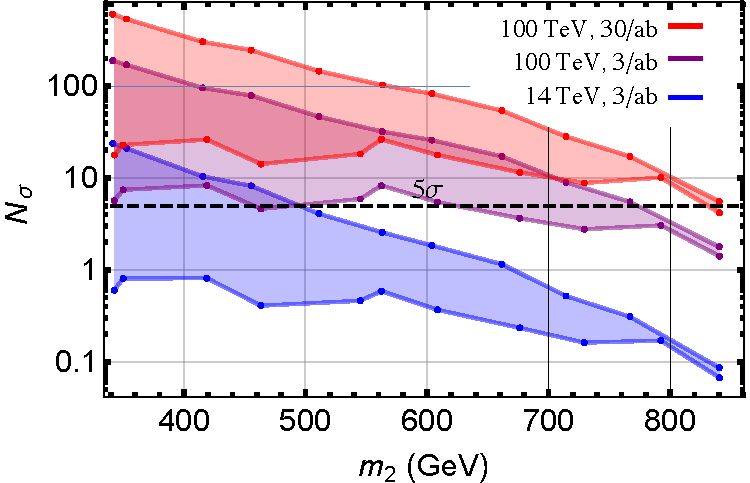
\includegraphics[width=0.49\linewidth]{\main/section3/plots/LogScale_Comb_bandPlot1.pdf}
    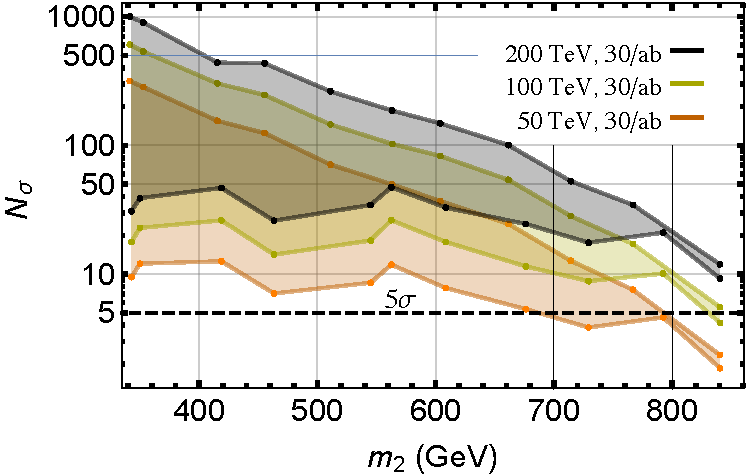
\includegraphics[width=0.49\linewidth]{\main/section3/plots/LogScale_Comb_bandPlot2.pdf}
    % 
    \caption{
    Discovery potential for the singlet-induced strong first order EWPT using resonant di-Higgs production combining 4\texttau\ and b\={b}\textgamma\textgamma\ final states\cite{Kotwal:2016tex}. Vertical axis gives significance as a function of the singlet-like scalar mass $m_2$. Left panel gives comparison of the reach for the HL-LHC (blue band) and the FCC-hh with 3 ab$^{-1}$ and 30 ab$^{-1}$ (purple and red bands, respectively). Right panel shows the prospective reach for different center of mass energies, assuming 30 ab$^{-1}$.    
        }
    \label{fig:ewpt_resdihiggs}
  \end{center}
\end{figure}

It is worth noting that the foregoing analyses are based on the assumption that the di-Higgs production process is dominated by the resonant amplitude. As discussed in Section 9.6.2, inclusion of interference with non-resonant amplitudes may lead to an enhanced sensitivity, particularly at higher values of the singlet-like mass $m_2$. The corresponding gain in going to the HE-LHC may be as much as a 40-50\% increase in mass reach compared to that of the HL-LHC, depending on the choice of other model parameters.

Another class of signatures providing important information about the couplings in the Higgs potential in singlet-extended Higgs sectors involves pair production of the new scalar itself. These processes can complement resonant di-Higgs production in their coverage of the parameter space. For example, the process $p p\rightarrow h_2 h_2 \rightarrow 3\ell 3\nu j j$ was analyzed in Ref.~\cite{Chen:2017qcz} and shown to provide good sensitivity to the first-order EWPT-compatible parameter space at both the high luminosity LHC and a future 100 TeV collider for masses below the di-Higgs threshold. While the analogous study has not been performed for the 27 TeV HE-LHC, $h_2 h_2$ production should still provide sensitivity to the couplings in the potential responsible for strengthening the EWPT, improving over the reach of the HL-LHC. In models in which a new $\mathbb{Z}_2$ symmetry is imposed on the singlet scalar, the VBF-like topology $p p \rightarrow j j h_2 h_2$ can be used to access the relevant Higgs portal coupling. In this case, $h_2$ is stable and escapes the detector as missing energy. Ref.~\cite{Curtin:2014jma} showed that this process at 100 TeV can probe first-order EWPTs for relatively low scalar masses. The analogous studies for the 14 TeV HL-LHC and 27 TeV HE-LHC remain to be done. 

Beyond direct production, the HE LHC will provide opportunities to observe indirect signatures of a strong first order EWPT through modifications of Higgs couplings. Considering first the xSM, the mixing between the doublet and singlet states will lead to modifications of the Higgs triple self coupling. This possibility is indicated in Fig.~\ref{fig:ewpt_self}, where we show he correlation between the critical temperature for the first order EWPT and the triple self coupling. The vertical axis gives the ratio of the xSM triple self-coupling of Higgs-like state $h_1$ to its Standard Model value, corresponding to the quantity $\kappa_\lambda$  introduced earlier in this chapter.  According to the analysis presented in the first part of Section~\ref{sec:THanetal}, a 15\% determination of $\kappa_\lambda$ may be possible using the $bb\gamma\gamma$ channel (however, see a parallel analysis later in that section for a less optimistic projection). This sensitivity corresponds roughly to the width of the green band in Fig.~\ref{fig:ewpt_self}. One can see that there exists a wide range of xSM parameter choices that would lead to an observable deviation of $\kappa_\lambda$ with the HE LHC.

\begin{figure}[hbtp]
  \begin{center}
    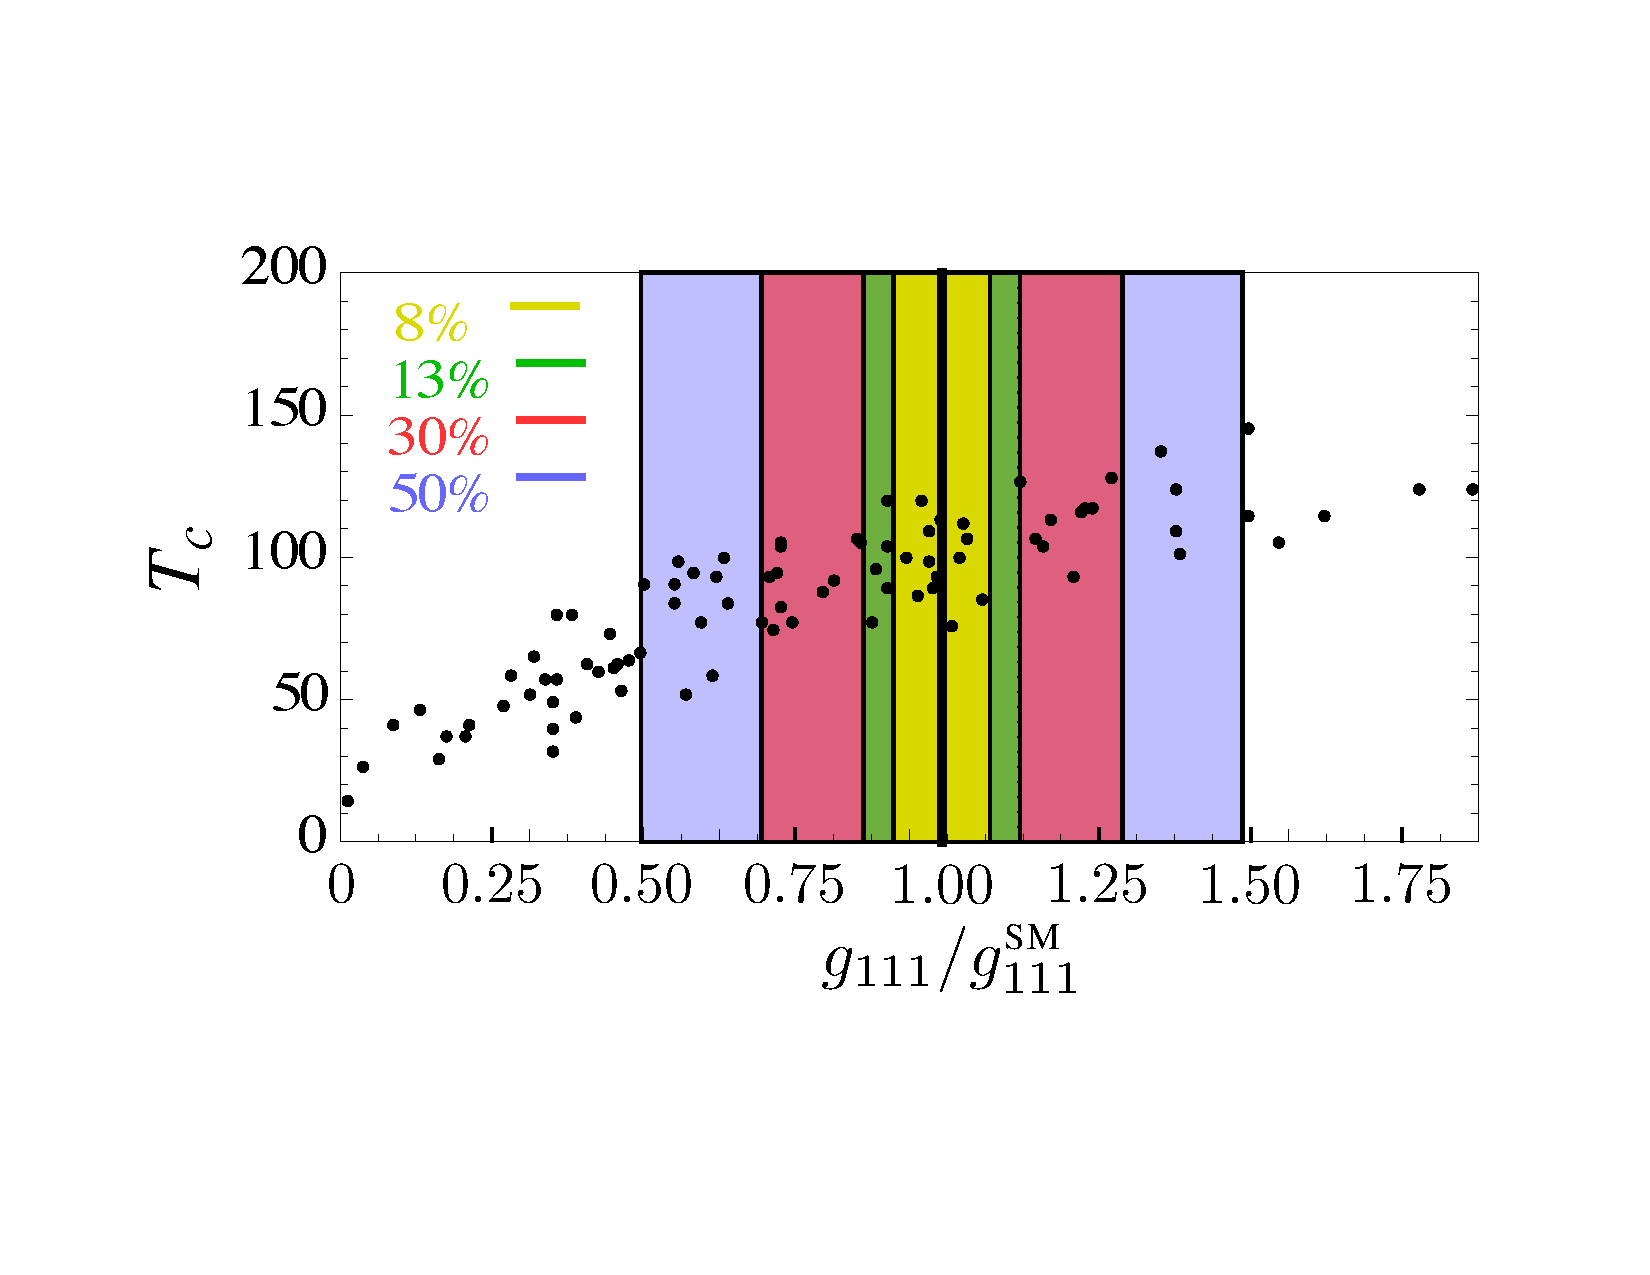
\includegraphics[width=0.49\linewidth]{\main/section3/plots/Self_Coupling--rescale_axis.pdf}
  %  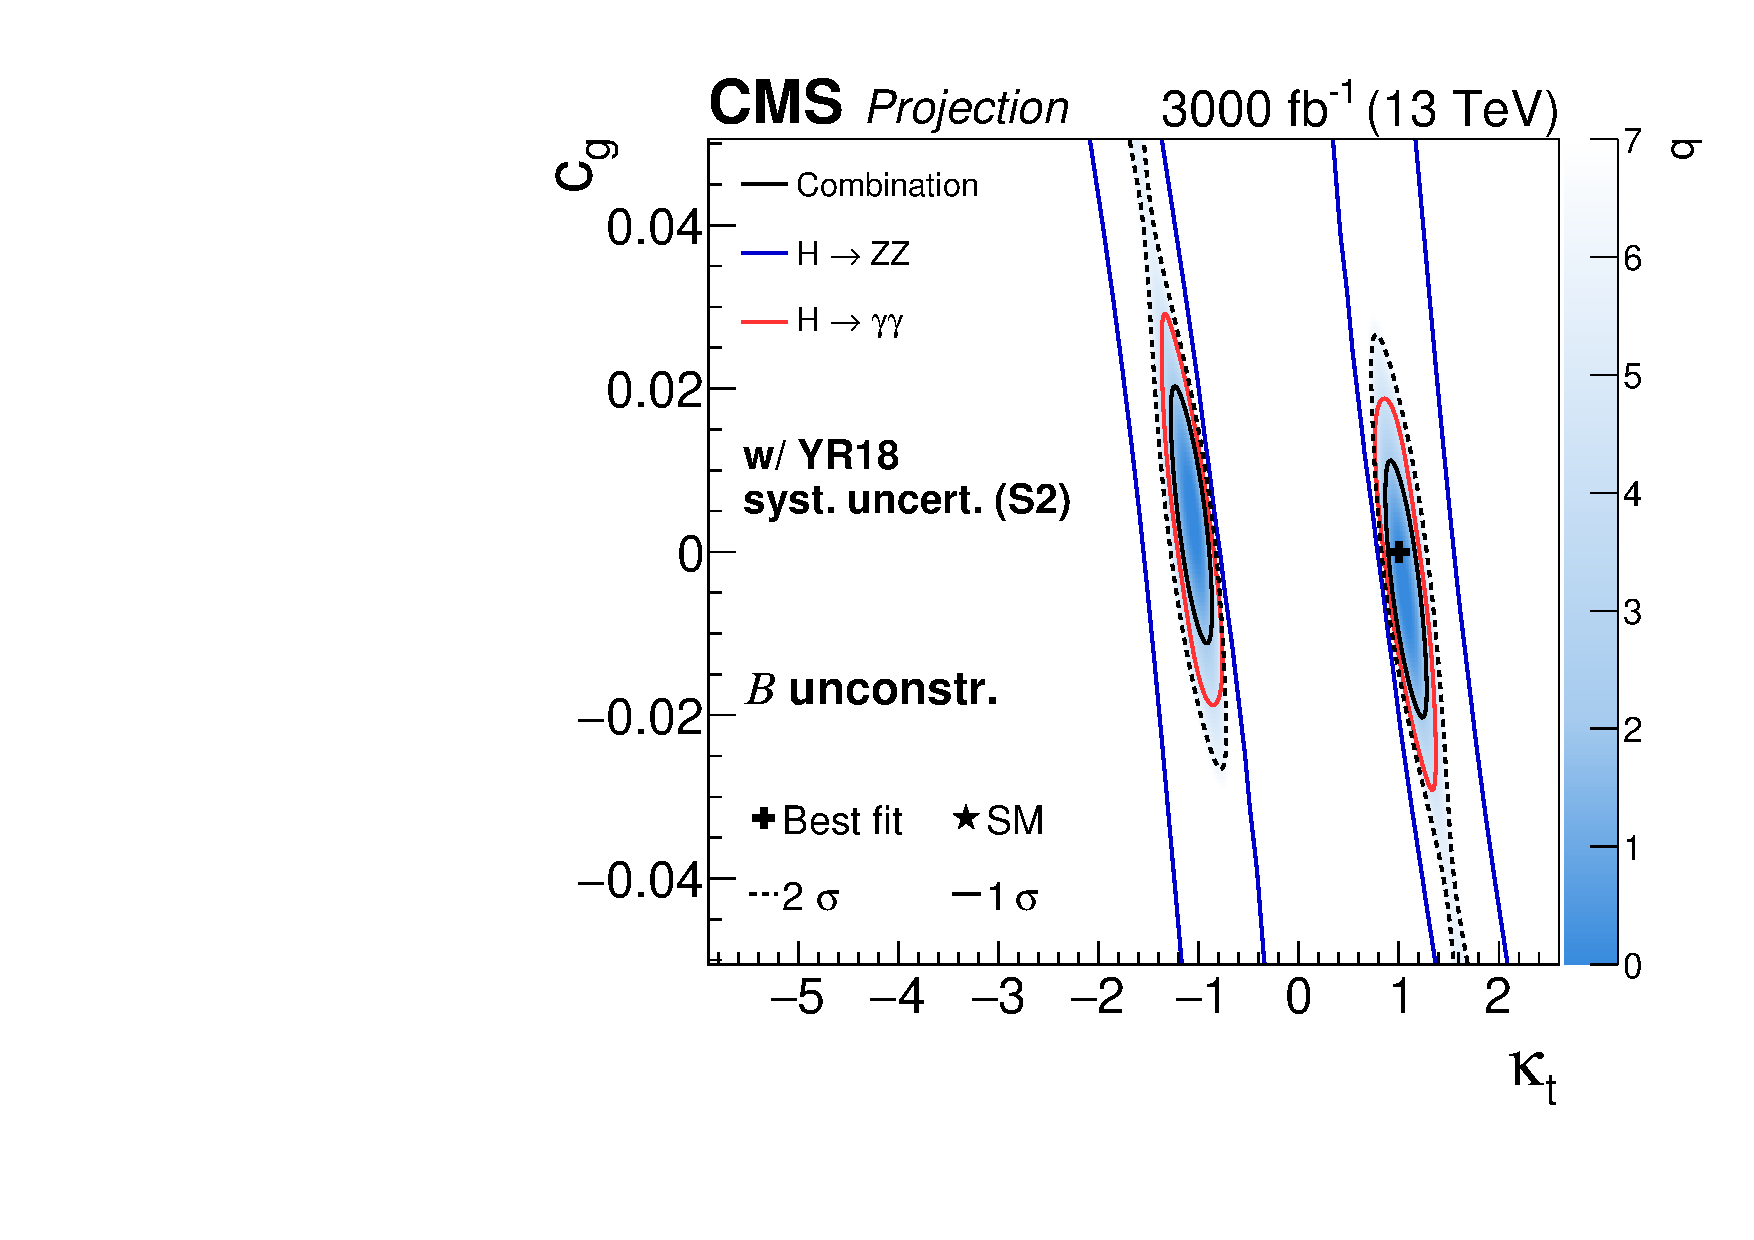
\includegraphics[width=0.49\linewidth]{\main/section2/plots/differentials/projection_ktcg_plot_floatingBRs_scenario2.pdf}
    % 
    \caption{
    Parameter space scan for a singlet model extension of the Standard Model. The points indicate a first order phase transition. These points lead to signals observable at future colliders. Shown is the correlation between critical temperature $T_c$ (vertical axis) and the triple Higgs ($h_1 h_1 h_1$) coupling scaled to its SM value (horizontal axis). SM prediction for the latter is indicated as $g_{111}/g_{111}^\mathrm{SM}=1$. Adapted from Ref.~\cite{Profumo:2014opa}   
        }
    \label{fig:ewpt_self}
  \end{center}
\end{figure}

\begin{figure}[hbtp]
  \begin{center}
  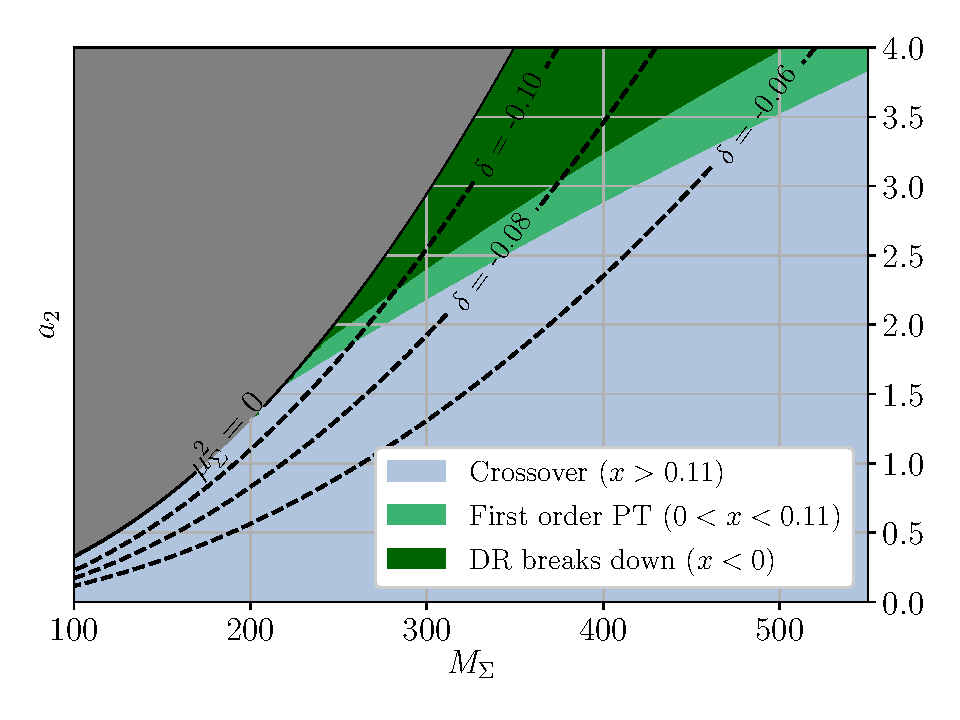
\includegraphics[width=0.49\linewidth]{\main/section3/plots/Triplet_EWPT.pdf}
    % 
    \caption{
    EW phase diagram for the real triplet extension of the SM scalar sector. Horizontal axis gives the triplet mass and vertical axis indicates the triplet-Higgs coupling. Light blue and green regions correspond to cross-over and first order transitions. Dark green (\lq\lq DR breaks down") and grey regions indicate parameter choices for which the present non-perturbative computations are not applicable. Dashed lines indicate relative shift $\delta$ in the Higgs diphoton decay rate compared to its Standard Model value. From Ref.~\cite{Niemi:2018asa}.    
        }
    \label{fig:ewpt_triplet}
  \end{center}
\end{figure}

Going beyond the SM, one may also anticipate a strong first order EWPT in scalar sector extensions carrying electroweak charge. Among the most widely studied ones, such scenario is the 2HDM. The authors of Refs.~~\cite{Dorsch:2013wja,Dorsch:2014qja} have shown that the strong phase transition would be correlated with the presence of the\linebreak $\rm A^0\to Z H^0$ decay and that a nearly definitive probe of this possibility could be achieved with the LHC. An interesting alternative is a scalar EW triplet with vanishing hypercharge.Interactions between the latter and the Standard Model doublet could lead to breaking of electroweak symmetry through either a single transition to the Higgs phase or through a succession of transitions\cite{Patel:2012pi}. Recently, the latter possibility has been explored in Ref.~\cite{Niemi:2018asa} using non-perturbative methods. In this work, it is shown how a precise measurement of the Higgs diphoton decay rate could probe the nature of the transition in this scenario. Fig.~\ref{fig:ewpt_triplet} illustrates this possibility. The horizontal and vertical axes give the triplet mass and coupling to the Higgs boson, respectively. The light blue and green regions correspond to a cross-over transition and first order phase transition, respectively. The dashed lines indicate the relative reduction in the Higgs diphoton decay rate relative to the prediction for the Standard Model. When combined with knowledge of the triplet mass, a precise measurement of the diphoton decay rate would indicate whether the transition is first order or crossover. As shown in Fig. 30, one expects to achieve a 1.8\% ($1\sigma$) determination of the Higgs-diphoton coupling parameter $\kappa_\gamma$ with the HL-LHC.
%For a 5$\sigma$ observation, a measurement of $\Gamma($H$\to$\textgamma\textgamma) at the anticipated FCC precision would be needed.



